\subsection{Supported magnitude-frequency distributions}
The magnitude-frequency distributions currently supported by the 
\gls{acr:oqe} are the following: 
\begin{description}
    \item[A discrete incremental magnitude-frequency distribution] \hfill \\
    It's the simplest distribution supported. It's defined by the 
    minimum value of magnitude (representing the mid point of the first
    bin) and the bin width. 
    The distribution itself is simply a sequence of floats describing the 
    annual number of events for different bins. The maximum magnitude 
    admitted by this magnitude-frequency distribution is just the sum of 
    the minimum magnitude and the product of the bin width by the number 
    annual rate values.

    Below we provide an example of the xml that should
    be incorporated in a seismic source description in order to define 
    this \gls{acr:mfd}. An additional example for this distribution can
    be also found at page \pageref{example_incremental_mfd}.
\begin{Verbatim}[frame=single, commandchars=\\\{\}, fontsize=\footnotesize]
<incrementalMFD minMag="5.05" binWidth="0.1">
    <occurRates>0.15 0.08 0.05 0.03 0.015</occurRates>
</incrementalMFD>
\end{Verbatim}
    This is the magnitude-frequency distribution obtained with the above
    settings is represented in Figure \ref{fig:evenly_discretized_mfd}.
% ..............................................................................
% . . . . . . . . . . . . . . . . . . . . . . . . . . . . . . . . . . . > Figure
\begin{figure}[!ht]
\centering
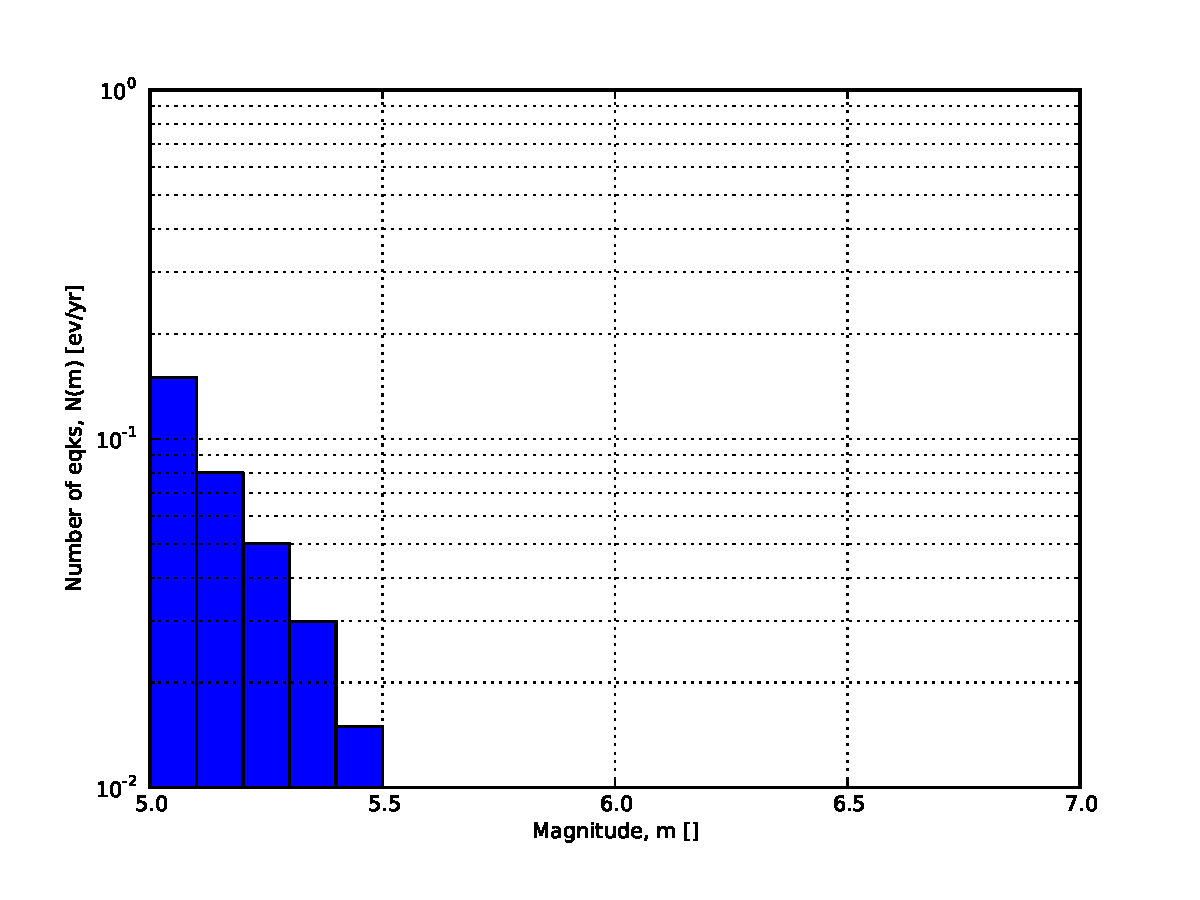
\includegraphics[width=12cm]{./figures/hazard/ed_mfd.pdf}
\caption{Example of an incremental magnitude-frequency distribution.}
\label{fig:evenly_discretized_mfd}
\end{figure}
% . . . . . . . . . . . . . . . . . . . . . . . . . . . . . . . . . . . < Figure
% ..............................................................................
%
\item[A double truncated Gutenberg-Richter distribution] \hfill \\
    This distribution is de\-scribed by means of a minimum \texttt{minMag}
    and maximum magnitude \texttt{maxMag} and by the $a$ and $b$ values 
    of the Gutenberg-Richter relationship. 
    
    The syntax of the xml used to describe this magnitude-frequency 
    distribution is rather compact as demonstrated in the following example
\begin{Verbatim}[frame=single, commandchars=\\\{\}, fontsize=\footnotesize]
<truncGutenbergRichterMFD aValue="5.0" bValue="1.0" minMag="5.0" 
        maxMag="6.0"/>
\end{Verbatim}

    Figure \ref{fig:dt_gr_mfd} shows the magnitude-frequency distribution 
    obtained using the parameters of the considered example.
% ..............................................................................
% . . . . . . . . . . . . . . . . . . . . . . . . . . . . . . . . . . . > Figure
\begin{figure}[!ht]
\centering
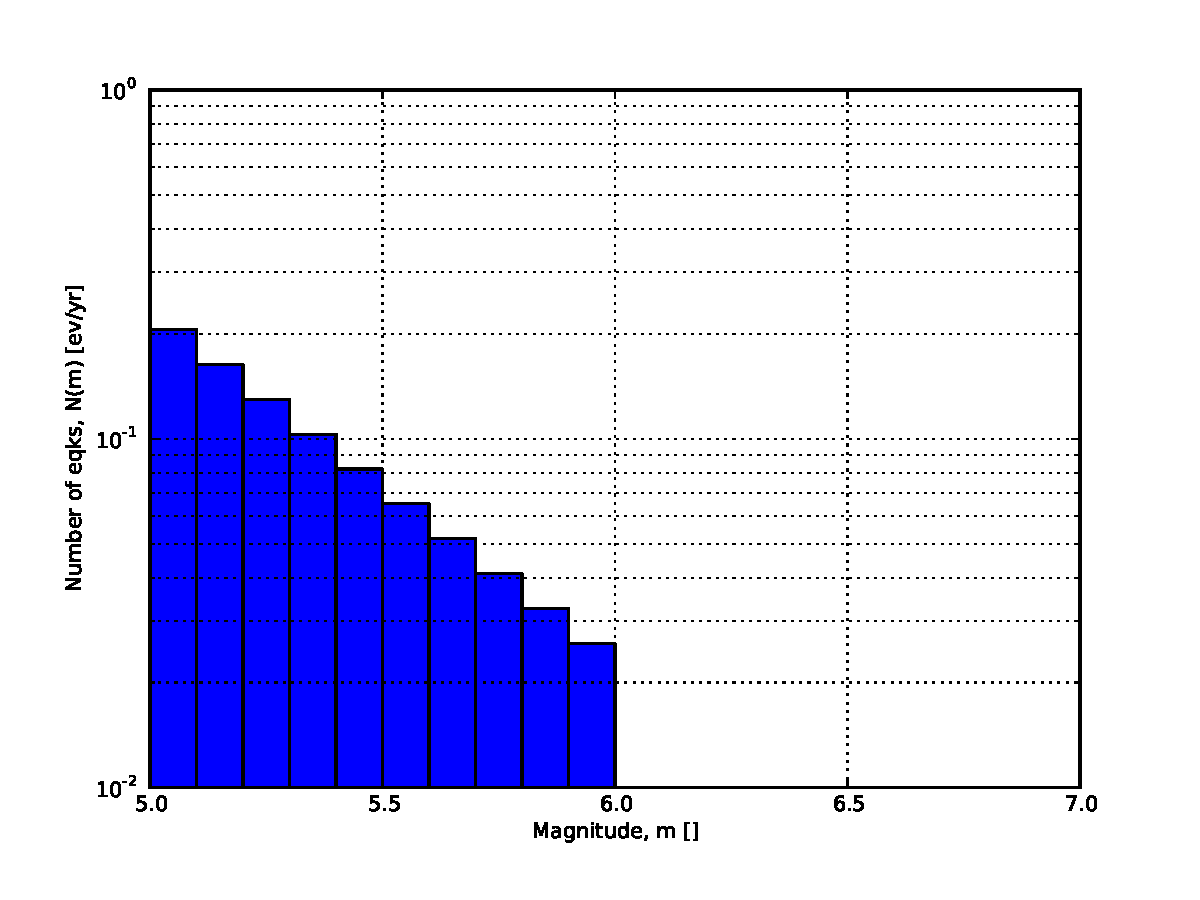
\includegraphics[width=12cm]{./figures/hazard/dt_mfd.pdf}
\caption{Example of a double truncated Gutenberg-Richter 
magnitude-frequency distribution.}
\label{fig:dt_gr_mfd}
\end{figure}
% . . . . . . . . . . . . . . . . . . . . . . . . . . . . . . . . . . . < Figure
% ..............................................................................
%
%
%\item[Characteristic earthquake model (\`{a} la \cite{youngs1985})]
%    In \citexear{youngs1995}, \citeauthor{youngs1995}
%\begin{Verbatim}[frame=single, commandchars=\\\{\}, fontsize=\footnotesize]
%    AA
%\end{Verbatim}
%% ..............................................................................
%% . . . . . . . . . . . . . . . . . . . . . . . . . . . . . . . . . . . > Figure
%\begin{figure}[!ht]
%\centering
%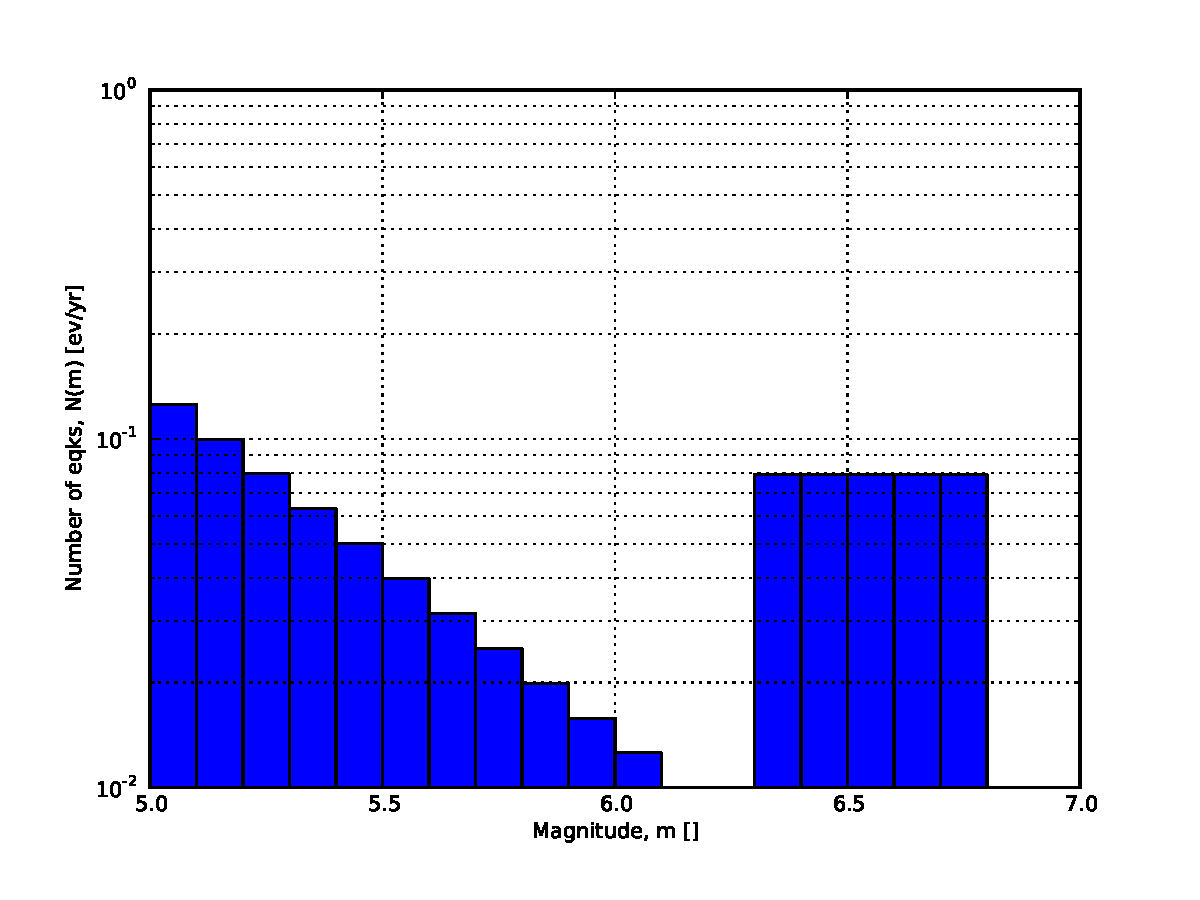
\includegraphics[width=12cm]{./figures/hazard/yc_mfd.pdf}
%\caption{\cite{youngs1985} magnitude-frequency distribution.}
%\label{fig:yc_gr_mfd}
%\end{figure}
% . . . . . . . . . . . . . . . . . . . . . . . . . . . . . . . . . . . < Figure
% ..............................................................................

\end{description}
